\chapter{Конструкторский раздел}

\section{Этапы решения поставленной задачи}

Исходными данными для задачи является описание диаграммы деятельности с помощью XMI. По этому описанию строится UML диаграмма и преобразуется в простую сеть Петри. Для построения раскрашенной сети из описания диаграммы выделяются используемые переменные и строится предварительное описание типов. После задания пользователем начальной разметки на основе предварительных данных о типах переменных строится окончательное множество типов и раскрасок. И с учетом видимости переменных выстраивается раскраска сети. Общий процесс функционирования представлен на рис. \ref{fig:fig1}. 

\begin{figure}
	\begin{center}
		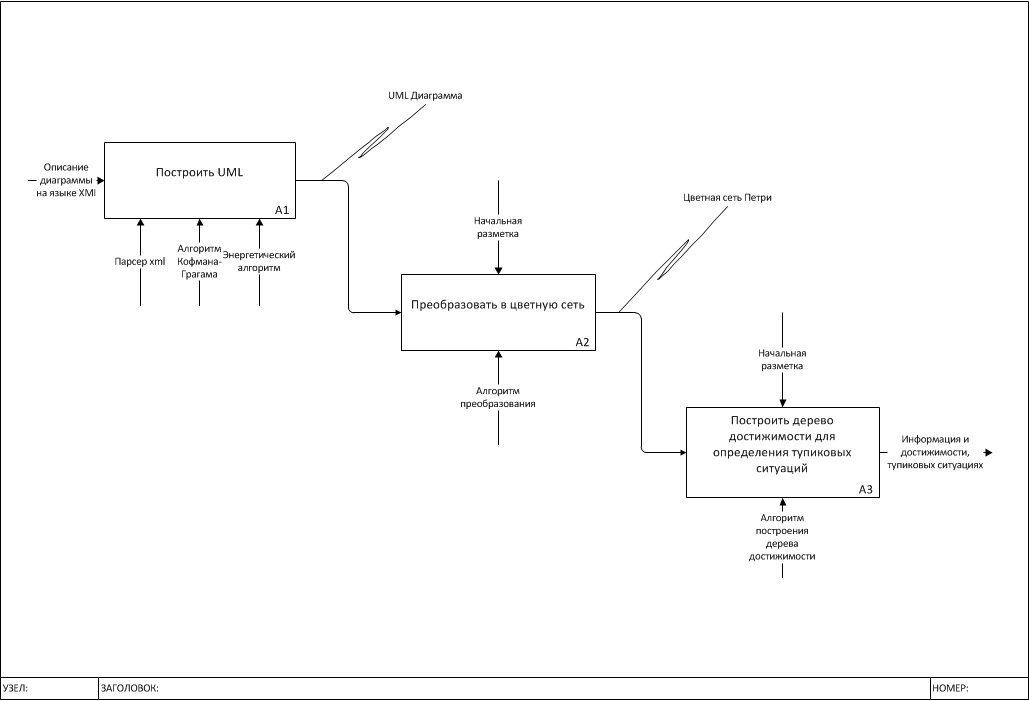
\includegraphics[width=\textwidth]{include/IDEF0.png}
	\end{center}
	\caption{Общий процесс функционирования.}
	\label{fig:fig1}
\end{figure}

Диаграмма деятельности представляет собой граф, вершины которого обозначают действия, а дуги ~--- переходы от одного действия к другому. Способы преобразования UML-диаграмм в простую сеть Петри широко известны, но для преобразования в раскрашенную сеть одних данных диаграммы не хватает: для раскрашенной сети необходимо сформировать множество типов и определить раскраски вершин (т.е. определить тип входных переменных). Процесс преобразования в раскрашенную сеть Петри представлен на рис. \ref{fig:fig2}.

\begin{figure}
	\begin{center}
		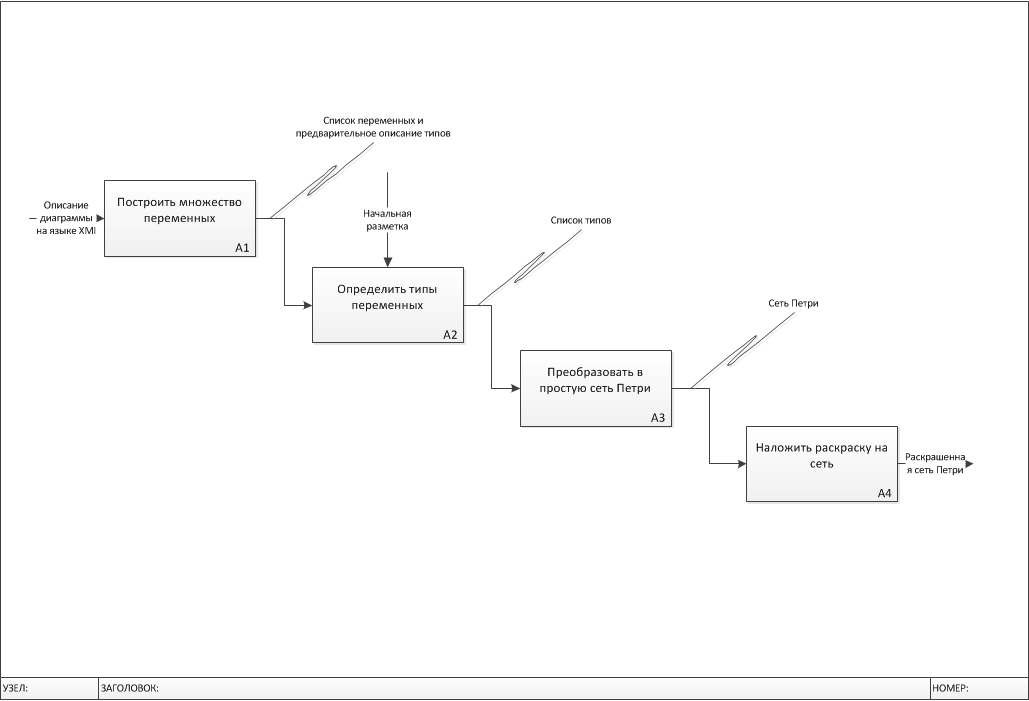
\includegraphics[width=\textwidth]{include/IDEF0ColouredPetri.png}
	\end{center}
	\caption{Процесс преобразования UML диаграммы деятельности в раскрашенную сеть Петри.}
	\label{fig:fig2}
\end{figure}

\section{Построение диаграммы деятельности}

\subsection{Алгоритм Кофмана-Грагама}

\subsection{Энергетический алгоритм}

\section{Описание UML диаграмм с помощью XMI}

Для описания диаграммы деятельности используется стандарт XMI. Каждая вершина имеет имя, тип и уникальный идентефикатор, описанные как аттрибуты, и список входных и выходных вершин. Иднтефикатор используется для связи между вершинами и переходами. Если вершина имеет тип \textit{action}, то она может содержать описание действий, по которым в дальнейшем будет выстраиваться множество переменных.

Каждый переход имеет строго одну исходящую и входящую вершину и может содержать в себе правила защиты перехода (например, для условного перехода \textit{condition}).

Основываясь на описанных правилах, получим структуру описания диаграммы:

\begin{lstlisting}[style=grammar,basicstyle=\small,caption={Структура XMI файла}]
<activity_diagram>
	<states>
		<state id, name, type>
			<incoming transitions>
			<outgoing transition>
			<action>
		</state>
	</states>
	<transitions>
		<transition id>
			<source state>
			<target state>
			<guard>
		</transition>
	</transitions>
<activity_diagram>
\end{lstlisting}

\section{Преобразование диаграммы деятельности в раскрашенную сеть Петри}

Наибольшей сложностью в процессе преобразования диаграммы в раскрашенную сеть Петри является формирование самой раскраски сети. Не существует четких правил, по которым можно определить достаточность раскраски, а так же возникает проблема избыточности, при которой сформированная сеть не будет точно моделировать работу диаграммы или не будет работать вовсе из-за невозможности совершения перехода.

Сам алгоритм построения раскрашенной сети Петри можно разделить на четыре этапа:

\begin{enumerate}
\item[1.] построение списка используемых переменных по описание диаграммы;
\item[2.] задание начальной разметки и формирование множества типов для соотвествующих переменных;
\item[3.] преобразование диаграммы в простую сеть Петри;
\item[4.] формирование раскраски сети с учетом начальной разметки и границ видимости переменных.
\end{enumerate}

Исходя из общих правил формирования множества раскрасок, необходимо каждое составное действие разделить на объект, субъект и само действие (\ref{fig:fig4}).

\begin{figure}
	\begin{center}
		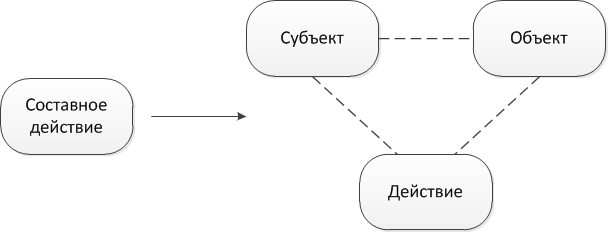
\includegraphics[width=0.6\textwidth]{include/CompositeActivity.png}
	\end{center}
	\caption{Треугольник сложного действия.}
	\label{fig:fig4}
\end{figure}

Сначала выделяются субъект и объект действия. Если на объект действия накладываются условные ограничения (не всегда может быть доступен, например, канал передачи данных, свободный блок оперативной памяти и т.п.), его необходимо отделить от субъекта действия, так как в сети Петри он будет обеспечивать второе условие для срабатывания перехода действия. Субъект и объект действия в общем случае связаны правилом, в соответствии с которым это действие происходит. \cite{Korotkov} 

\subsection{Получение списка переменных}

На первом этапе построение раскрашенной сети необходимо рассмотреть множество переменных, описывающих работу диаграммы. Условимся, что если переменные (в любой части описания переменной) имеют одинаковые имена, то они имеют и одинаковые типы.

На основе этого мы можем построить предварительное описание типов. Предположим, что на диаграмме имеются три блока действия:
\begin{enumerate}
\item[1.] player.cell = field.cell;
\item[2.] player.resource = player.resoure + field.resource;
\item[3.] player.resource = player.resoure - resource.
\end{enumerate}

По этому описанию можно заключить, что в системе фигурируют три переменные: player, field и resource, причем первые две имеют составной тип. Так же получаем то, что типы player и resource имет одинаковое описание типов: $ { cell, resource } $, причем тип всех переменных resource одинаковый. Таким образом, после первого этапа анализа получаем:

\begin{lstlisting}[style=grammar,basicstyle=\small]
player : struct { cell, resource }
field : struct { cell, resource }
resource : simple type
\end{lstlisting}

\subsection{Введение начальной разметки}

На втором этапе пользователю предлагается задать входные данные для диаграммы, основываясь переменных, выделенных на пером этапе. Основываясь на этих значениях, можно построить заключение о типах переменных. Остановим выбор на трех простейших типах: \textit{integer}, \textit{boolean}, \textit{string}, из которых можно образовывать кортежи и сложные структуры.

Для примера, приведенного на первом этапе, построим множество типов:

\begin{lstlisting}[style=grammar,basicstyle=\small]
player : [ ((1, 1), 0) ]
field : [ ((1, 2), 2); ((1, 3), 1); ((2, 1), 1); ... ]
resource : 1
\end{lstlisting}

Учитывая предварительное описание типов, получаем

\begin{lstlisting}[style=grammar,basicstyle=\small]
player : struct { cell : (int * int), resource : int }
field : struct { cell : (int * int), resource : int }
resource : int
\end{lstlisting}

\subsection{Преобразование в простую сеть Петри}

Диаграмма деятельности во многом подобна сетям Петри. Но в сетях Петри действия моделируются переходами, а на диаграмме деятельности узлами. Кроме того, если в диаграмме деятельности движение фишки необходимо приостановить, то это делается между узлами на дугах, а не внутри блока. Таким образом, правильный перевод в сеть Петри заменяет узлы на переходы, а дуги на позиции. Узлы диаграммы представляются по-разнову, в зависимости от типа (\ref{fig:fig5}):

\begin{figure}
	\begin{minipage}[h]{0.5\linewidth}
		\center{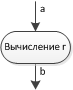
\includegraphics[scale=1]{include/Activity.png}}
	\end{minipage}
	\hfill
	\begin{minipage}[h]{0.4\linewidth}
		\center{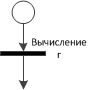
\includegraphics[scale=1]{include/ActivityPetri.png}}
	\end{minipage}
	\hfill
	\begin{minipage}[h]{1\linewidth}
		\begin{tabular}{ p{0.5\linewidth} p{0.5\linewidth} }
			\centering 1. & \centering 2. \\
		\end{tabular}
	\end{minipage}
	\hfill	
	
	\begin{minipage}[h]{0.5\linewidth}
		\center{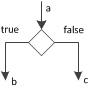
\includegraphics[scale=1]{include/Condition.png}}
	\end{minipage}
	\hfill	
	\begin{minipage}[h]{0.4\linewidth}
		\center{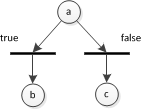
\includegraphics[scale=1]{include/ConditionPetri.png}}
	\end{minipage}
	\hfill
	\begin{minipage}[h]{1\linewidth}
		\begin{tabular}{ p{0.5\linewidth} p{0.5\linewidth} }
			\centering 3. & \centering 4. \\
		\end{tabular}
	\end{minipage}
	\hfill		
	
	\begin{minipage}[h]{0.5\linewidth}
		\center{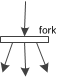
\includegraphics[scale=1]{include/Fork.png}}
	\end{minipage}
	\hfill	
	\begin{minipage}[h]{0.4\linewidth}
		\center{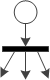
\includegraphics[scale=1]{include/ForkPetri.png}}
	\end{minipage}
	\hfill	
	\begin{minipage}[h]{1\linewidth}
		\begin{tabular}{ p{0.5\linewidth} p{0.5\linewidth} }
			\centering 5. & \centering 6. \\
		\end{tabular}
	\end{minipage}
	\hfill		
	
	\begin{minipage}[h]{0.5\linewidth}
		\center{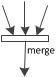
\includegraphics[scale=1]{include/Merge.png}}
	\end{minipage}
	\hfill
	\begin{minipage}[h]{0.4\linewidth}
		\center{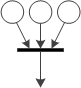
\includegraphics[scale=1]{include/MergePetri.png}}
	\end{minipage}
	\begin{minipage}[h]{1\linewidth}
		\begin{tabular}{ p{0.5\linewidth} p{0.5\linewidth} }
			\centering 7. & \centering 8. \\
		\end{tabular}
	\end{minipage}
	\hfill		
	
	\caption{Преобразование узлов диаграммы деятельности в сеть Петри.  деятельность; 3,4 условие; 5,6 ветвление; 7,8 синхронизация.}
	\label{fig:fig5}
\end{figure}

Условия для принятия решения в сетях Петри задаются как свойства соответствующих переходов. Позиция, предшествующая ветвлению, имеет два выхода, и маркер позиции перейдет через тот переход, условию которого удовлетворяет его значение. Стоит отметить потенциальную возможность ошибок, предупреждение которых целесообразно рассматривать как одно из формальных правил.
\begin{itemize}
\item Если для переходов ветвления не заданы условия их срабатывания, возникает неопределенность, в какую ветку перейдет маркер.
\item В случае если ни одно из условий не является истинным, переход становится недоступным ~--- маркер остается в своей позиции.
\end{itemize}

\subsection{Наложение раскраски}

На последнем этапе необходимо получить раскраску сети. Раскраска характеризуется кортежом типов. Главной проблемой является формирование множества состояний, принадлежащих некоторому типу.

Если стартовую разметку содержит не только начальная вершина, но и вершина, имеющая входные дуги, то для выходного перехода из этой вершины добавляется еще одна вершина, не имеющая входных дуг, и содержащая разметку.

Будем считать, что тип, сформированной старторой разметкой начальной вершины присущ какждой вершине, которая достижима из нее. Раскраски остальных вершин, отличных от начальной будем выводить следующим образом: если вершина содержит некоторую переменную, то для всех путей, для которых встречается эта переменная, формируется новый цвет, состоящий из типа текущей раскраски и типа переменной.

\section{Алгоритм построения дерева достижимости}

Алгоритм начинает свою работу с определения начальной разметки. До тех пор, пока имеются граничные вершины, они обрабатываются алгоритмом.

Пусть x – граничная вершина, которую необходимо обработать, и с которой связана разметка $ \mu(x) $.
\begin{enumerate}
\item Если в дереве имеется другая вершина y, не являющаяся граничной, и с ней связана разметка $ \mu(y) = \mu(x) $, то вершина x дублируется. 
\item Если для разметки $ \mu(x) $ ни один из переходов неразрешим, т.е. $ \mu(x) $ тупиковая разметка, то x терминальная вершина.
\item Для любого перехода $ t_{j} $, из множества T разрешенного в разметке $ \mu(x) $, создать новую вершину z дерева достижимости. Разметка $ \mu(z) $, связанная с этой вершиной, определяется для каждой позиции $ p_{i} $ следующим образом:
\begin{enumerate}
\item если $ \mu(x)_{i} = \omega, то \mu(z)_{i} = \omega $;
\item если на пути от корневой вершины к x существует вершина y такая, что $ \mu(y)\rightarrow^{t_{j}} \mu(x), \mu(y) < \mu(x) и \mu(y)_{i} < \mu(x)_{i} $, то $ \mu(z)_{i} = \omega $;
\item в противном случае $ \mu(z)_{i} = \mu(x)_{i} $.
\end{enumerate}

\end{enumerate}

Дуга, помеченная $ t_{j} $, направлена от вершины х к вершине z. Вершина x переопределяется как внутренняя, вершина z становится граничной. Когда все вершины дерева становятся терминальными, дублирующими или внутренними, алгоритм останавливается. Из алгоритма построения дерева достижимости следуют следующие выводы:
\begin{itemize}
\item сеть ограничена тогда и только тогда, когда символ $ \omega $ отсутствует в дереве;
\item сеть безопасна, если число фишек в каждой позиции не превышает 1;
\item сеть живая, если в дереве отсутствуют циклы и тупики.
\end{itemize}

\label{cha:design}